\documentclass[11pt, a4paper]{article}

\usepackage{titling}
\usepackage{multirow}
\usepackage{graphicx}
\usepackage{caption}

\newcommand{\subtitle}[1]{%
  \posttitle{%
    \par\end{center}
    \begin{center}\large#1\end{center}
    \vskip0.5em}%
}

\newcommand{\specialcell}[2][c]{%
  \begin{tabular}[#1]{@{}l@{}}#2\end{tabular}}
  
\setlength{\oddsidemargin}{0.5cm}
\setlength{\evensidemargin}{0.5cm}
\setlength{\topmargin}{-1.6cm}
\setlength{\leftmargin}{0.5cm}
\setlength{\rightmargin}{0.5cm}
\setlength{\textheight}{24.00cm} 
\setlength{\textwidth}{15.00cm}
\parindent 0pt
\parskip 5pt
\pagestyle{plain}
\usepackage[numbers]{natbib}
\usepackage{capt-of}
\usepackage{graphicx,url}

\begin{document}

\title{CITS3401 Data Exploration \& Mining Project 1}
\subtitle{Healthy Burgers Fast Food Chain}
\author{Aleck Greenham 20362627 \\ Ash Tyndall 20915779}
\date{26th April 2013}

\maketitle

\section*{Abstract}

This document details the design of a data cube suitable for the \textit{Healthy Burgers} franchise, a fast-food restaurant chain with stores in three countries, to aid management in its plans for improving sales and global expansion. Where the system requirements \cite{designdoc} were ambiguous or incomplete, reasonable assumptions were made and documented.

\section*{Introduction}

The client, Healthy Burgers, wishes to mine historical sales data from their nine stores spread across three countries in Australasia to aid management in making decisions regarding global expansion of the franchise and improving sales at existing restaurants. Each restaurant maintains a Online Transaction Processing (OLTP) database and there are aggregate databases at the state, country and worldwide levels. The company maintains data on sales, products, suppliers and restaurants. The purpose of this document is to detail the design of a data cube to extract data from these databases that will support the decisions faced by Healthy Burgers management.

\section*{Limitations}

It is outside the scope of this assessment to address the importing of data from the heterogeneous OLTP restaurant databases, including the cleaning of data. It shall be assumed that the data is complete, easily available and in the desired formats. It is acknowledged, however, that this would not be the case in real industry applications.

A detailed interpretation of the results of the OLAP operations is also outside the scope of this assessment. It falls to Healthy Burgers management to fully interpret and make recommendations or decisions based on the data stored within the data warehouse.

\section*{Requirements}

Table \ref{tab:requirements} is a summary of authors' interpretation of the initial requirements:

\begin{table}

\begin{tabular}{|l|l|l|}

\hline
\textbf{Object} & \textbf{Properties} & \textbf{Restrictions} \\
\hline

Country & & Australia, New Zealand, Singapore \\
\hline

\multirow{3}{3cm}{Store} & Interior Design  & 3 restaurants in each country \\
 	& Facility Type & 3 different interior designs \\
	& & Facilities are `dine in', `drive through' and `both' \\
\hline

\multirow{3}{3cm}{Combo Meal} & Price Category & 6 different combo meals \\
	& Calorie Value & Not all stores have combo meals \\
	& Products & Divided into 3 different price categories \\ 

\hline

\multirow{2}{3cm}{Supplier} & & There are 2 suppliers \\ 
	& & Suppliers do 3 combo meals each\\
\hline

\multirow{2}{3cm}{Sale} & Date & Date Between 2008 and 2012 \\
	& Combo &  \\
\hline

\multirow{2}{3cm}{Sales Period} & & Has 2 combo meals \\ 
	& & Can be `breakfast', `lunch' or `dinner' \\
\hline	

Promotional Period & & 6 promotional periods per year\\

\hline

\end{tabular}

\caption{System Requirements Summary}
\label{tab:requirements}

\end{table}

\subsection*{Assumptions}

The following assumptions were made:

\begin{itemize}
	\item To make the initial requirements \cite{designdoc} sufficiently complete
	\item To make the design scenario as realistic as possible 
	\item For the sake of simplicity or clarity (where realism was impossible, impractical or outside the scope of assessment)
\end{itemize}

\begin{enumerate}
	\item The type of ingredients are not important, only their supplier - i.e. the supplier is a proxy for how desirable the ingredients they supply are. 
	\item There are six combo meals globally.
	\item There are 3 sales periods, each with 2 combo meals, and only 6 combo meals to choose from. If it's true that not all stores sell all the combo meals, then some combo meals must be shared between sales periods.
	\item All non-combo products sold are not of interest (because they have no relation with any of the other data fields).
	\item The same suppliers provide the ingredients for same combo meals, globally.
	\item A promotional period has it’s own 6 combo meals (thus the combo meals change every 2 months).
	\item The price of combo meals is set at the store level.
\end{enumerate}

\section*{Schema Design}

A Star Schema was chosen as the design document \cite{designdoc} states Healthy Burgers is only interested in sales, which removes the need to have multiple fact tables (i.e. a Constellation Schema). Table \ref{tab:dimensions} shows the dimension tables used in the solution implementation.

The time values have been split into a number of different dimensions to facilitate the comparison of different time periods against each other. An example query is comparing the total sales during each sales period (Breakfast, Lunch or Dinner) across each promotional period (1st promotion, 2nd promotion, etc.) to find out whether a promotion was particularly successful for a given sales period.

The remaining data has been split up into dimensions to accommodate queries that would be reasonably expected to be of interest to Healthy Burgers management. 

\begin{table}
\begin{minipage}{0.6\textwidth}
\begin{tabular}{| p{.4\textwidth} | p{.5\textwidth} |}
\hline
	\textbf{Dimension} & \textbf{Fields} \\
	\hline

	\multirow{2}{.2\textwidth}{Store} & store\_key \\
	& country \\
	\hline

	Design & design\_key \\ 
	\hline

	Facilities & facility\_key \\
	\hline

	SalesPeriod & sales\_period\_key \\
	\hline

	PromotionalPeriod & promotional\_period\_key \\
	\hline

	Years & years\_key \\
	\hline

	\multirow{2}{.2\textwidth}{Combos} & combo\_key \\
	& calories \\
	\hline

	Suppliers & supplier\_key \\
	\hline

	Price Range & price\_range\_key \\
	\hline

	Calorie Range & calorie\_range\_key \\
	\hline

	\end{tabular}
	\caption{Dimension Tables}
	\label{tab:dimensions}
	
\end{minipage}
\begin{minipage}{0.45\textwidth}
\begin{tabular}{| p{.25\textwidth} | p{.6\textwidth} |}
	\hline
	\textbf{Field Type} & \textbf{Field} \\
	\hline	
	\multirow{10}{.25\textwidth}{Dimension Keys} & store\_key \\
		& design\_key \\ 
		& facility\_key \\
		& sales\_period\_key \\
		& promotional\_period\_key \\
		& years\_key \\
		& combo\_key \\
		& supplier\_key \\
		& price\_range\_key \\
		& calorie\_range\_key \\
	\hline	

	Measures & total\_sales\_in\_dollars \\
	\hline

	\end{tabular}
	\caption{Fact Table}
	\label{tab:facts}
\end{minipage}
\end{table}

The requirements state that Healthy Burgers is only interested in a single measurement: sales in dollars; this is reflected in the fact table which consists of keys to all the of available dimensions, and the total sales in dollars.

\section*{Implementation}

\subsection*{Data Generation}

A Python script (\texttt{genvals.py}) authored by Tyndall generated random data that fit within the restrictions imposed by the initial requirements and what was considered realistic. Product names were generated from random dictionary words; product attributes such as price and calorie values were normally variate around a realistic mean and standard deviation. The rest of the data was similarly generated.

In an endeavour to make the data as realistic as feasibly possible, care was taken to influence it in a variety of sensible ways. Sales were positively correlated with increasing caloric content, and similarly correlated with decreasing price.
Different suppliers and store designs affect sales and countries enjoy different sales periods to different extents.

\subsection*{Data Import}

An Excel workbook (\texttt{data-import.xlsx}) was developed with two worksheets to handle the generation of the attribute structure required by Palo; data cleaning and categorisation; and fact insertion. You can see examples of their function in \texttt{create-structure.png} and \texttt{create-data.png}.

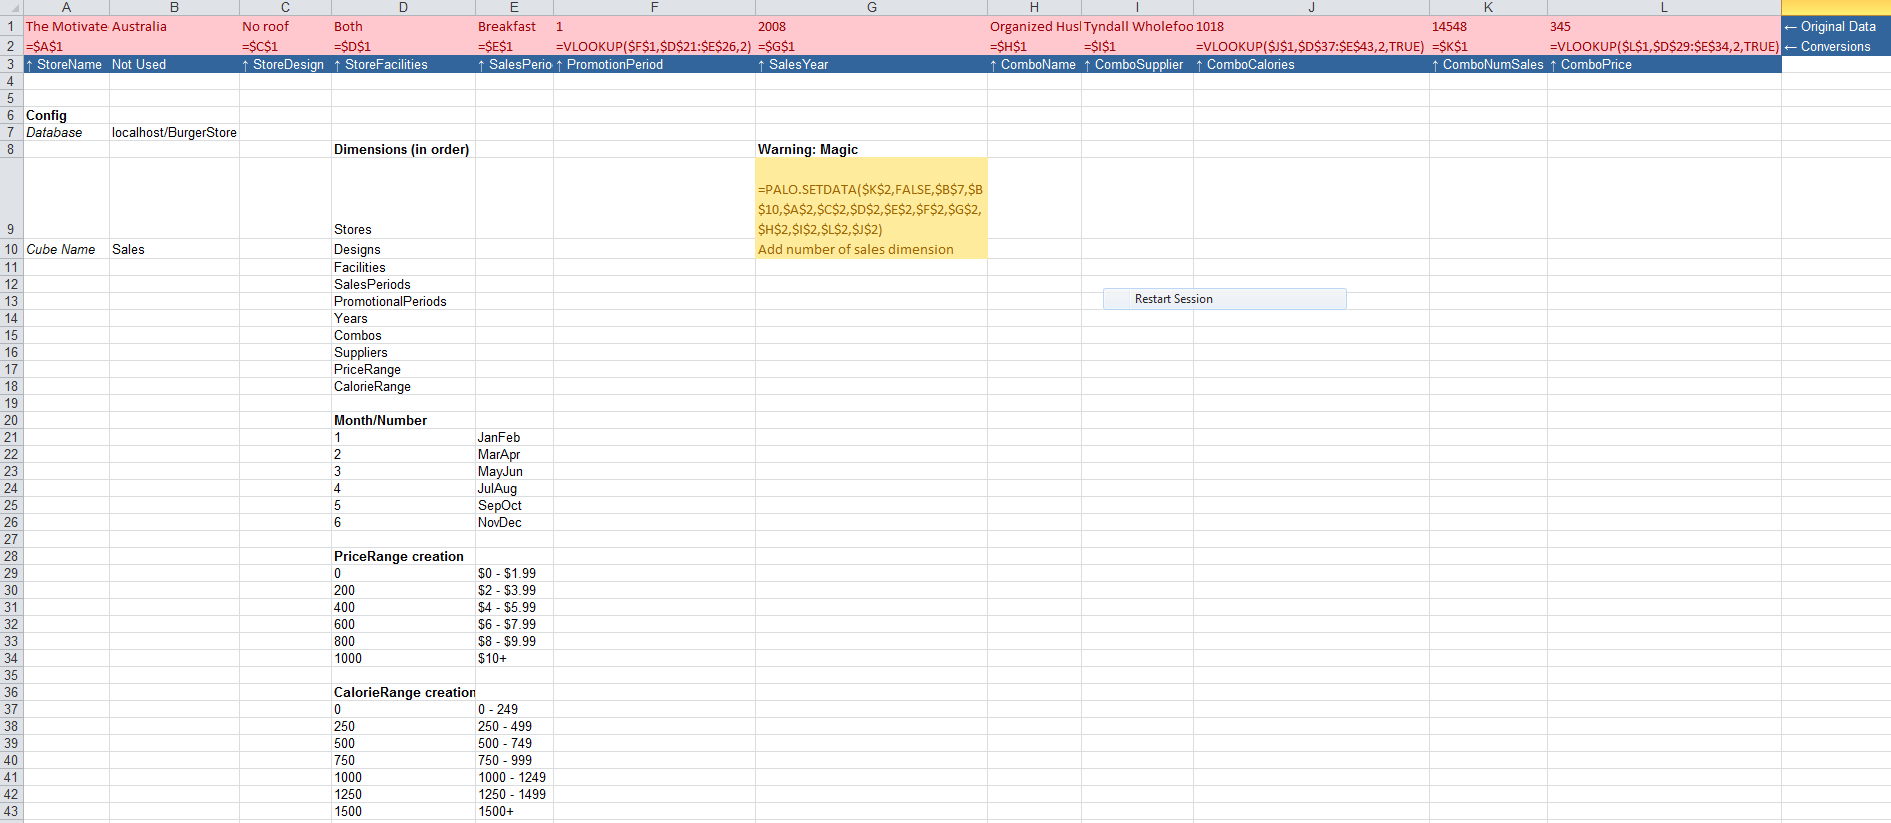
\includegraphics[width=15cm]{diagrams/create-data}

Palo's Import Wizard takes the input CSV file (\texttt{fulldata.csv}) generated by the Python script, and places it line-by-line in the first worksheet (``1. Create Structure'').
This worksheet's formulas are recalulated for each row as Palo iterates through them, and thus detects new categories as they appear in the data, creating the appropriate attributes and nesting structure in the OLAP database.

The Import Wizard is then used again on the second worksheet (``2. Create Data''). This worksheet then adds the Sales facts to the Sales data cube.

This 2-step process is necessary, as Palo strongly recommends against combining the \texttt{PALO.EADD} and \texttt{PALO.SETDATA} formulas in the same worksheet when using the Import Wizard.

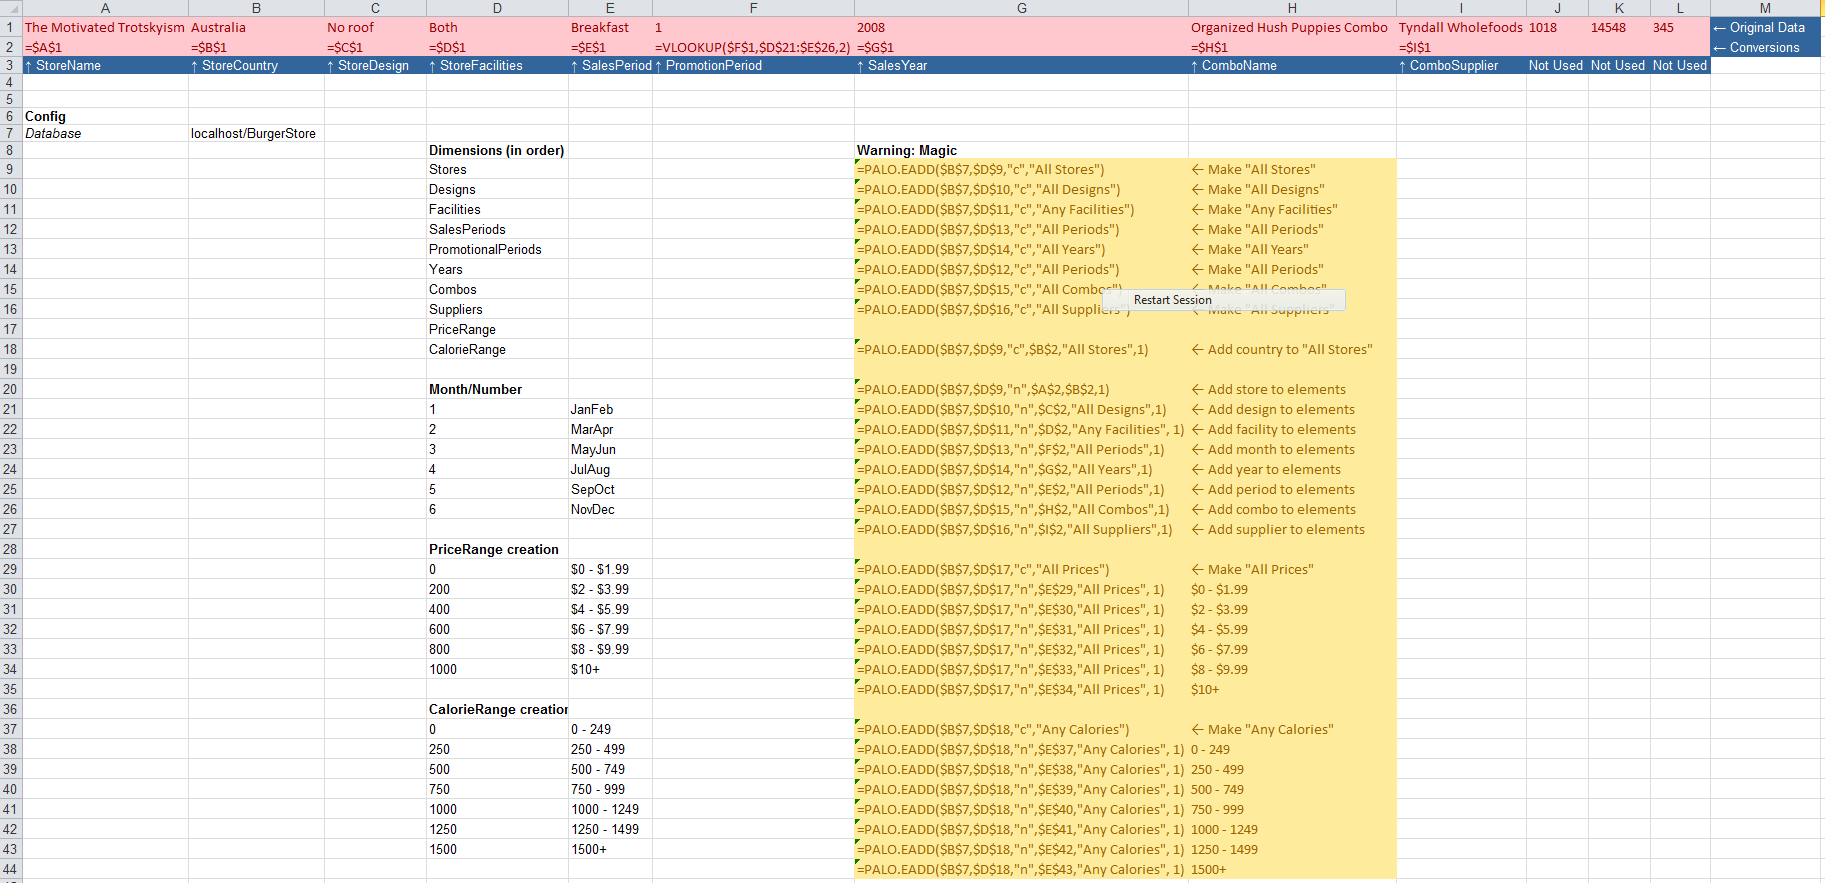
\includegraphics[width=15cm]{diagrams/create-structure}

\section*{Interesting Scenarios}

Scenarios were chosen for their perceived relevance and interest to Healthy Burgers management for their goals of expanding the Healthy Burgers franchise into other countries, and to replicate the success of existing stores and products where possible, to increase sales and popularity.

Accompanying screenshots for each scenario may be found in the Appendices. The reader should note that although these images are technically not full screen, they do include enough details to verify they are indeed legitimate outputs of the Palo server/Excel plugin. Electronic copies should also be available with this submission.

\subsection*{Total sales in dollars per year by facility type}

It is of interest to Healthy Burgers to know the facility types positively correlated with large amounts of sales to aid in the decision of what facilities to offer in new restaurants. It is also useful for deciding whether to expand existing restaurants to offer new facilities, or whether to close existing facilities because they do not warrant the additional cost of running them.

\subsection*{Total sales in dollars per year by interior design}

Similar to facility types, the correlation between interior designs and total sales can be used for deciding the layouts of new restaurants or whether or not to renovate existing branches to be consistent with the more profitable operations - if this is indeed deemed an important factor in their success.

\subsection*{Total sales in dollars per category of calories by price bracket}

If high calorie meals are indeed more popular - and the data should be consulted to confirm this suspicion - then it is of interest to Healthy Burgers to ascertain how much people are willing to pay per calorie when it comes in the form of the different meals offered in the combos. This can be used to anticipate the success and pricing of future meals offered at both existing and future restaurants, to maximise profits.

\subsection*{Total sales in dollars per products supplied by suppliers by year}

Essentially, this offers an indication of how much profit Healthy Burgers is making from the products whose ingredients are provided by each supplier. This will reveal any correlations or trends regarding consumer preference for the ingredients of one supplier over another. This may also be used to help shape the future pricing of products, identifying and meals or combos that are currently over or under priced.

\subsection*{Total sales in dollars per sales period by country}

Total sales per country is of obvious utility for expanding the franchises stores. Countries may be identified as having significantly large sales and prove a sound choice for future restaurants. Alternatively, it may be decided that these countries are saturated in terms of similar restaurants and future expansion should take place elsewhere.

\begin{thebibliography}{9}

\bibitem{designdoc}
	CITS3401 Data Exploration and Mining - Project 1,
	http://undergraduate.csse.uwa.edu.au/units/CITS3401/labs/proj1-2013.html
		
\end{thebibliography}

\bibliographystyle{IEEEtranN}

\appendix
\section{Total sales in dollars per year by facility type} 
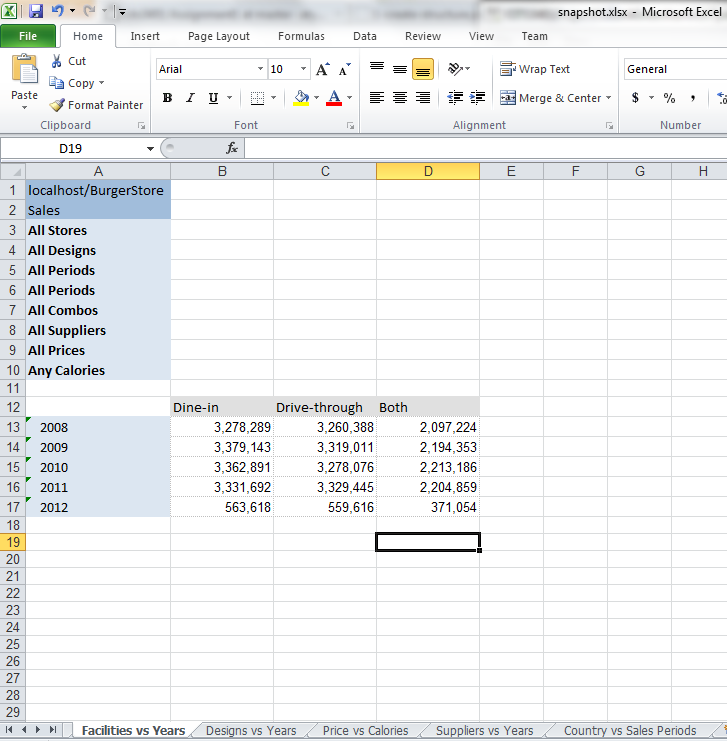
\includegraphics[width=15cm]{diagrams/FacilitiesVsYears}

\section{Total sales in dollars per year by interior design}
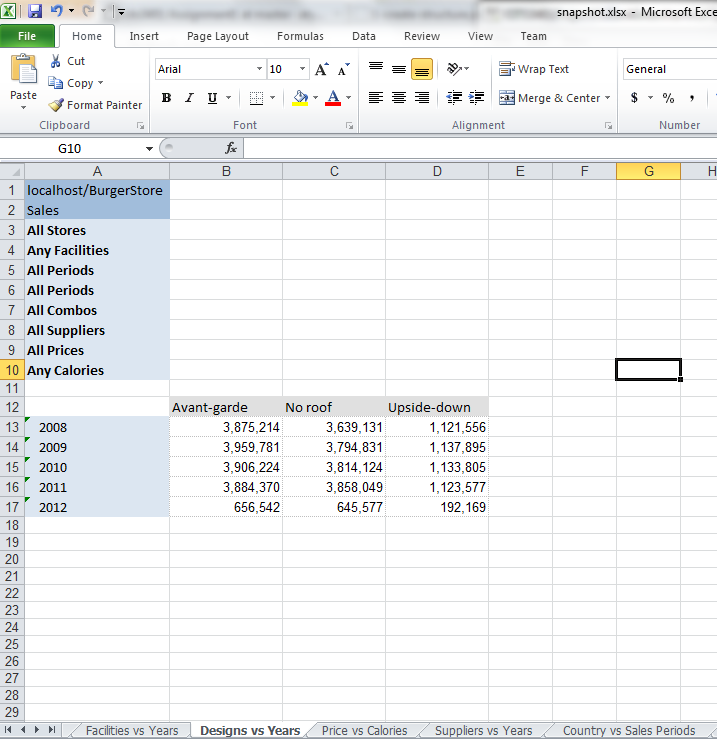
\includegraphics[width=15cm]{diagrams/DesignsVsYears}

\section{Total sales in dollars per category of calories by price bracket}
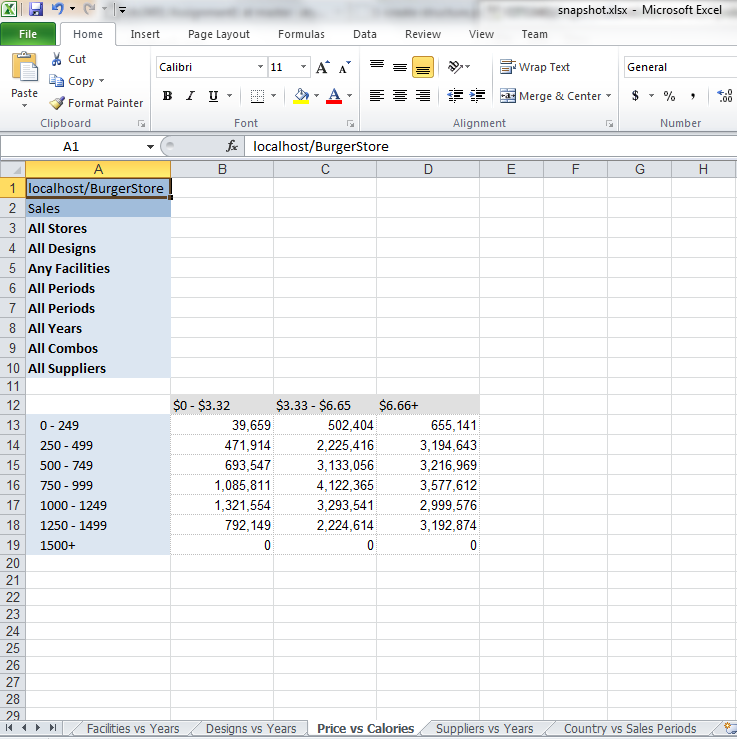
\includegraphics[width=15cm]{diagrams/PriceVsCalories}

\section{Total sales in dollars per products supplied by suppliers by year}
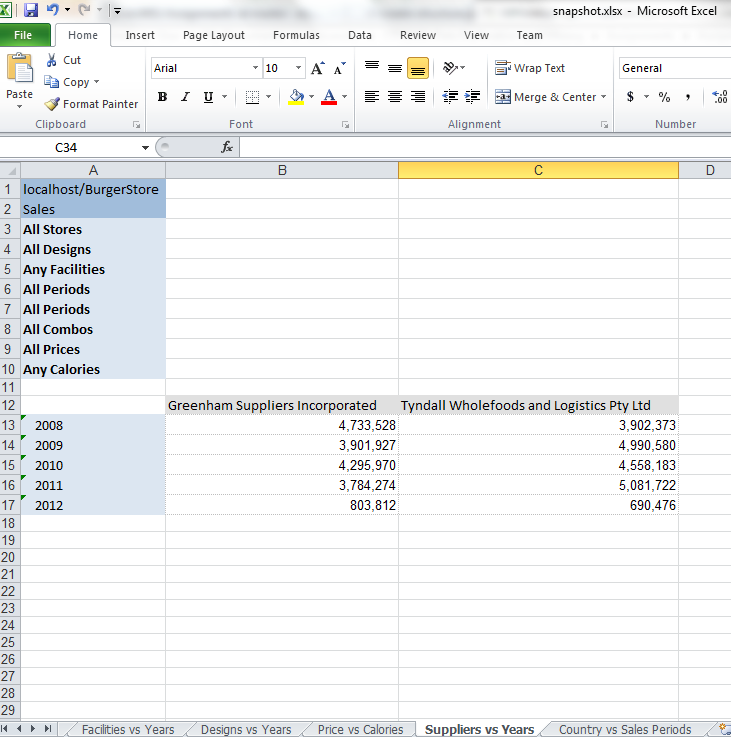
\includegraphics[width=15cm]{diagrams/SuppliersVsYears}

\section{Total sales in dollars per sales period by country}
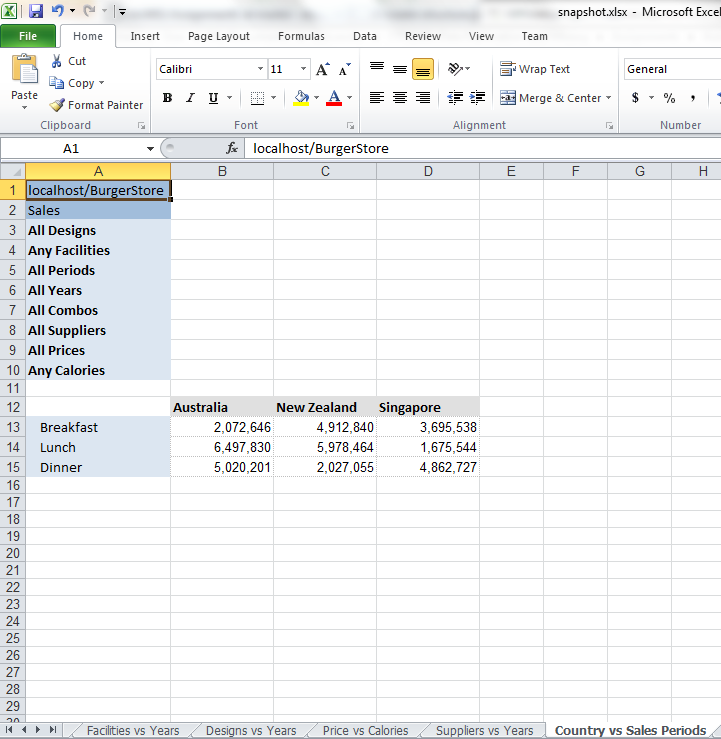
\includegraphics[width=15cm]{diagrams/CountryVsSalesPeriod}
\end{document}
